\documentclass[10pt]{beamer}
\usetheme{PaloAlto}
\usecolortheme{seahorse}
\setbeamertemplate{navigation symbols}{}
\setbeamertemplate{caption}[numbered]
%general package
%\usepackage[utf8]{inputenc}
\usepackage[english]{babel}
\usepackage{geometry}
\usepackage{tcolorbox}
\usepackage[export]{adjustbox}
\usepackage{graphicx}
\graphicspath{{../img}}

%math package
\usepackage{amsmath}
\usepackage{amsfonts}
%\usepackage{amssymb}
%\usepackage{amsthm}
%\usepackage{slashed}
%\usepackage{tikz-cd}

%font package
%\usepackage{mathrsfs}
%\usepackage{bm}

%misc. package
\usepackage{enumitem}

\author[B.H.]{{\Large MATH211 Calculus III}\\\vspace{6pt}Instructor: Ben Huang}
\date{}
\title[Section 11.4]{Section 11.4 Cross Product}
\institute[MU]{
\includegraphics[width = 0.382\textwidth]{MCLogo-Bck.png}}
\logo{
\includegraphics[scale = 0.3]{MCLogo-Bck.png}}
%general package
\usepackage[utf8]{inputenc}
\usepackage[english]{babel}
\usepackage{geometry}

%math package
\usepackage{amsmath}
\usepackage{amsfonts}
\usepackage{amssymb}
\usepackage{amsthm}
\usepackage{slashed}
\usepackage{tikz-cd}

%font package
\usepackage{mathrsfs}
\usepackage{bm}

%misc. package
\usepackage{enumitem}
\usepackage{tcolorbox}
\usepackage{etoolbox}
\usepackage{hyperref}
\hypersetup{
  colorlinks=true, urlcolor=blue
}




%declared operators
\DeclareMathOperator{\id}{Id}%identity
\DeclareMathOperator{\ind}{Ind\!}%index
\DeclareMathOperator{\tr}{Tr}%trace
\DeclareMathOperator{\e}{e}%exponential
\DeclareMathOperator{\im}{Im\!}%image
\DeclareMathOperator{\vol}{vol}%volume
\DeclareMathOperator{\cll}{\C\ell}%complexified Clifford algebra
\DeclareMathOperator{\gd}{\slashed{\partial}}%geometric Dirac
\DeclareMathOperator{\D}{\mathcal{D}}%generalized Dirac
\DeclareMathOperator{\Div}{div}%divergence
\DeclareMathOperator{\ud}{\,\mathrm{d}\!}

\DeclareMathOperator{\Hom}{Hom}
\DeclareMathOperator{\xd}{\,d\!}
\DeclareMathOperator{\curl}{curl}
\DeclareMathOperator{\dive}{div}


\newcommand{\norm}[1]{\lVert#1\rVert}
\newcommand{\R}{\mathbb R}
\newcommand{\vF}{\mathbf F}
\newcommand{\vv}{\mathbf v}
\newcommand{\inpr}[1]{\left\langle#1\right\rangle}
\newcommand{\fix}{(a,b)}
\newcommand{\uv}{\mathbf u}
\newcommand{\abs}[1]{\left\lvert #1\right\rvert}
%texting in citation
\makeatletter
\let\cite\relax
\DeclareRobustCommand{\cite}{%
  \let\new@cite@pre\@gobble
  \@ifnextchar[\new@cite{\@citex[]}}
\def\new@cite[#1]{\@ifnextchar[{\new@citea{#1}}{\@citex[#1]}}
\def\new@citea#1{\def\new@cite@pre{#1}\@citex}
\def\@cite#1#2{[{\new@cite@pre\space#1\if\relax\detokenize{#2}\relax\else, #2\fi}]}
\makeatother

\begin{document}

\frame{\titlepage}

\begin{frame}
\frametitle{Knowledge Checks}
Suppose $\mathbf u = u_1\mathbf i + u_2\mathbf j + u_3\mathbf k$, $\mathbf v = v_1\mathbf i + v_2\mathbf j + v_3\mathbf k$. What is the cross product $\mathbf u\times\mathbf v$?
\pause

\begin{tcolorbox}
$\mathbf u \times \mathbf v = (u_2v_3 - u_3v_2)\mathbf i + (u_3v_1 - u_1v_3)\mathbf j + (u_1v_2 - u_2v_1)\mathbf k.$
\end{tcolorbox}
\pause
What is the special relation between the directions of $\mathbf u \times \mathbf v$ and $\mathbf u$ or $\mathbf v$?\pause
\begin{tcolorbox}
$\mathbf u \times \mathbf v$ is orthogonal to both $\mathbf u$ and $\mathbf v$.
\end{tcolorbox}
\end{frame}

\begin{frame}
\frametitle{Knowledge Checks}
How is $\lVert\mathbf u\times\mathbf v\rVert$ related to  $\lVert\mathbf u\rVert$, $\lVert\mathbf v\rVert$, and  $\theta$?
\begin{figure}
\centering
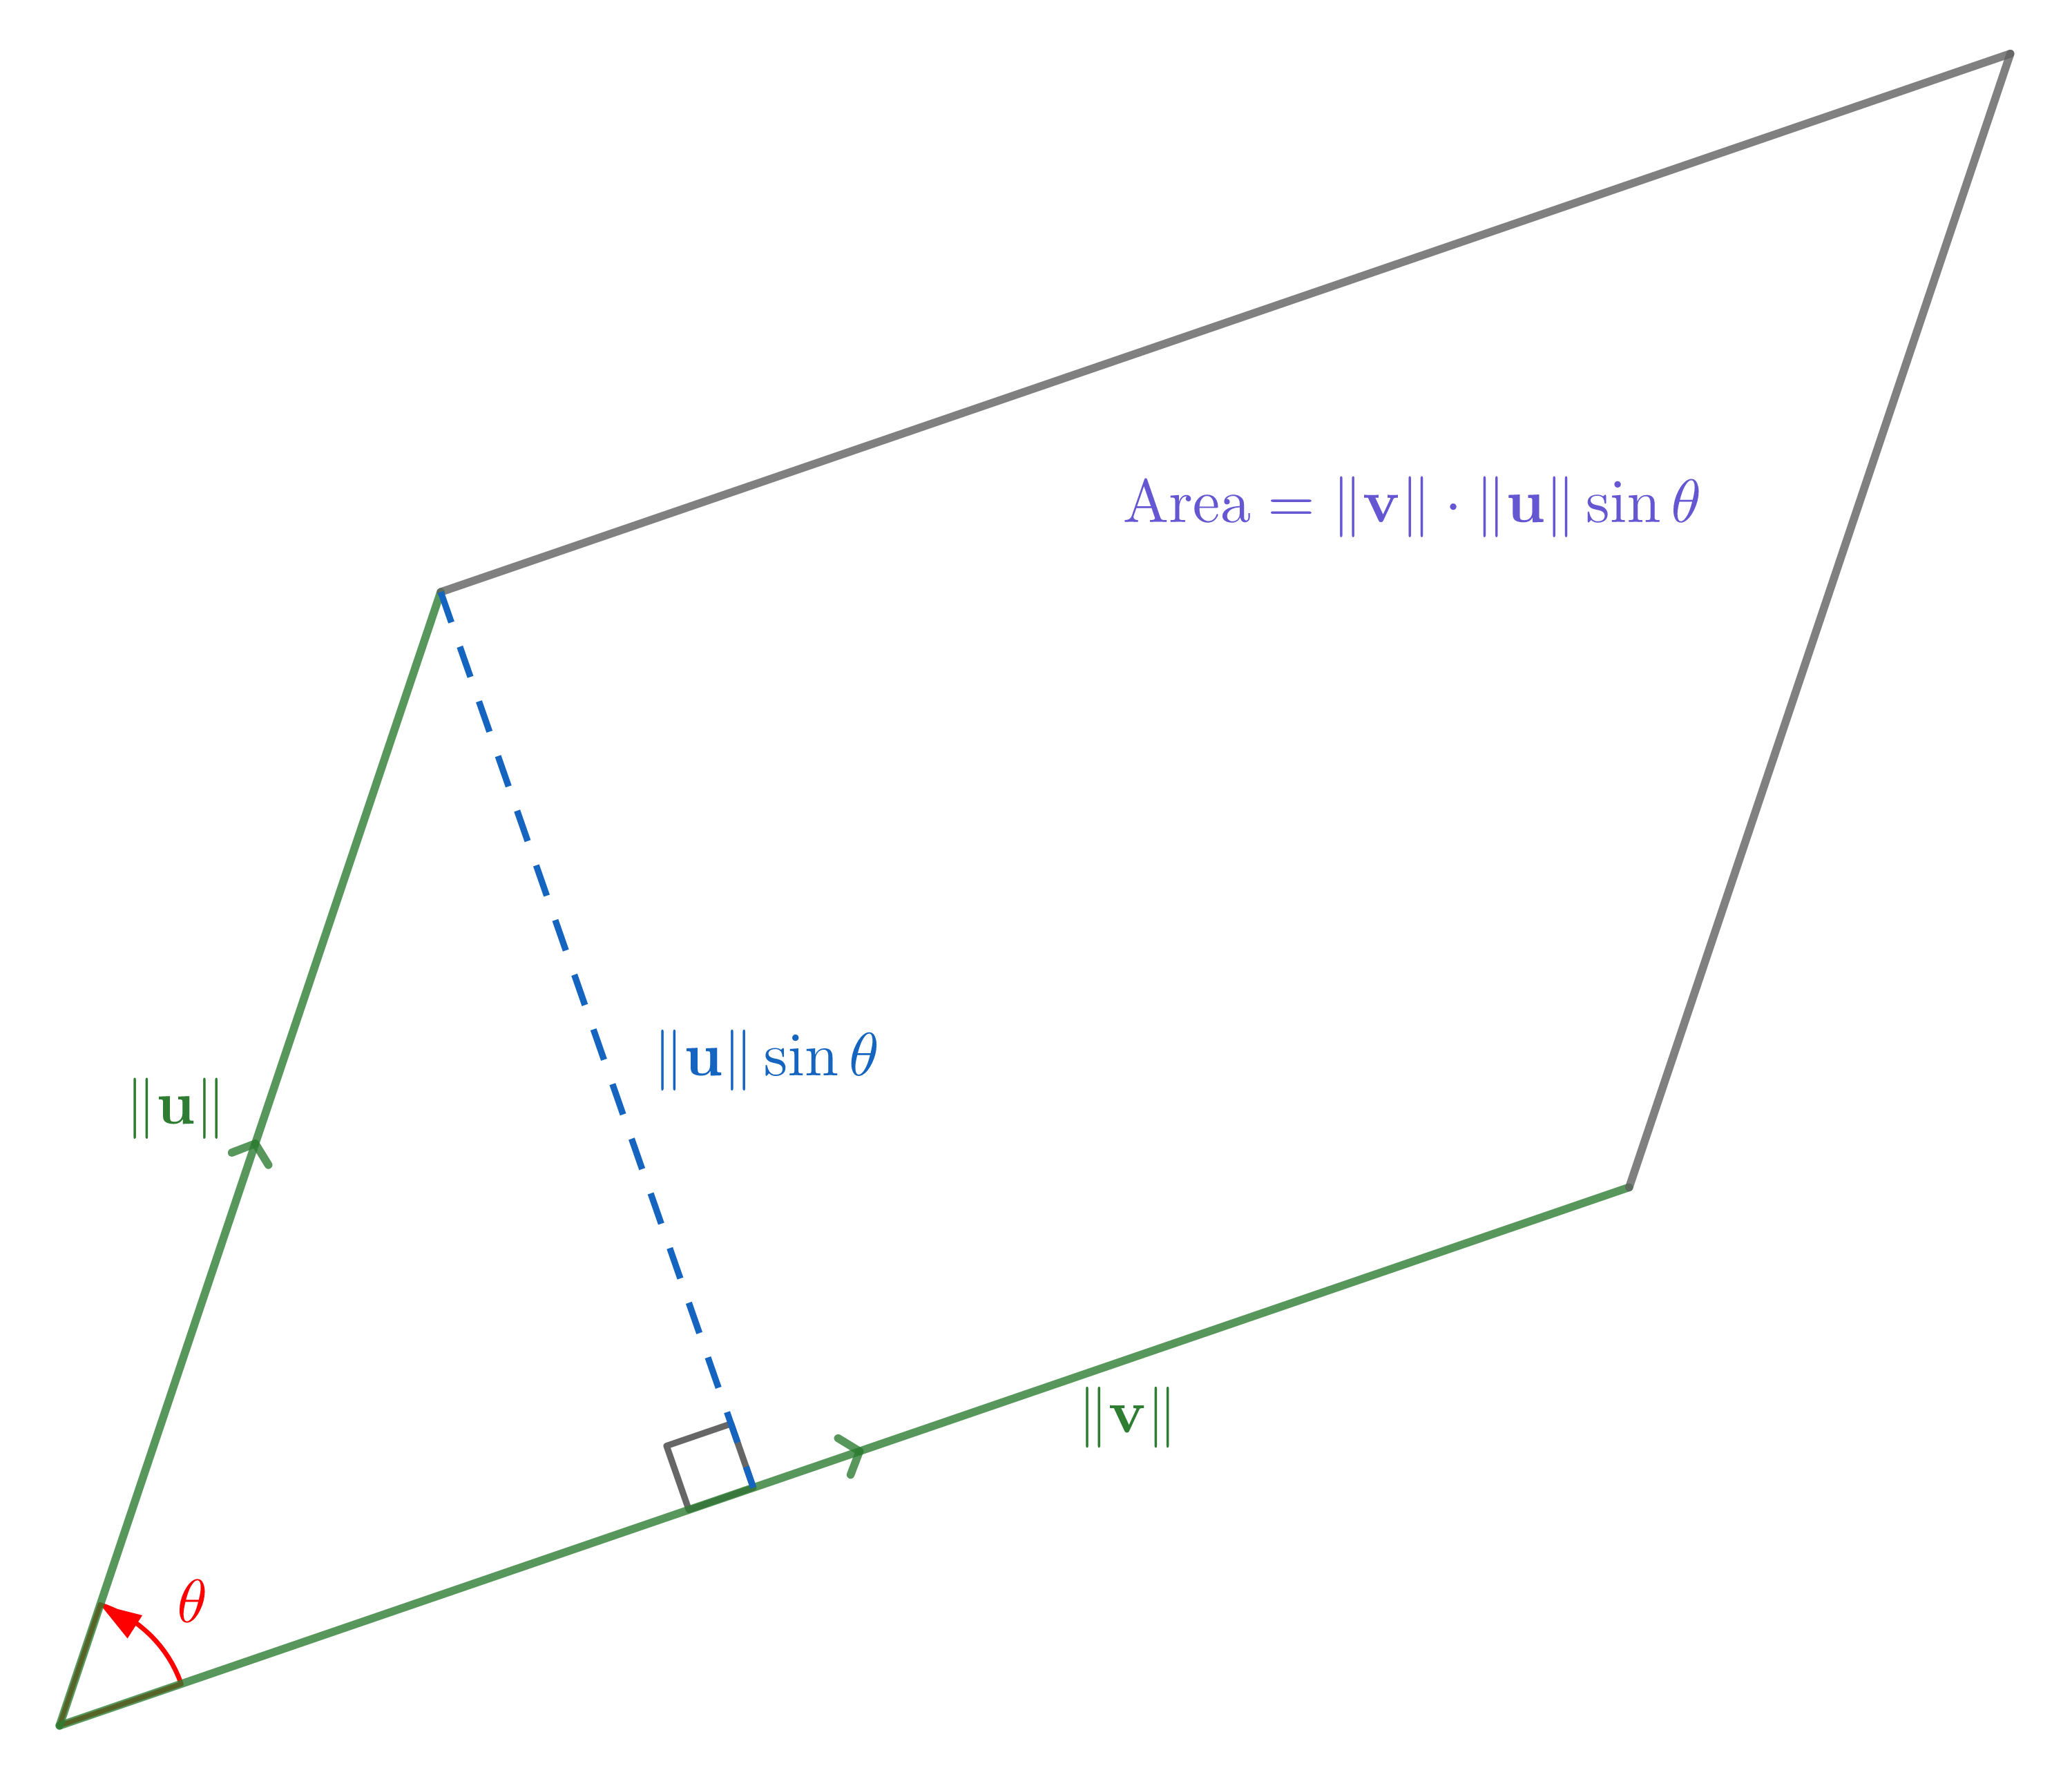
\includegraphics[width=0.618\textwidth]{area.png}
\end{figure}
\pause
\begin{tcolorbox}
$\lVert\mathbf u\times\mathbf v\rVert = \lVert\mathbf u\rVert\ \lVert\mathbf v\rVert \sin\theta = \text{the area of the parallelogram}$.
\end{tcolorbox}
\end{frame}

\begin{frame}
\frametitle{Knowledge Checks}
What is the torque?
\begin{tabular}{cc}
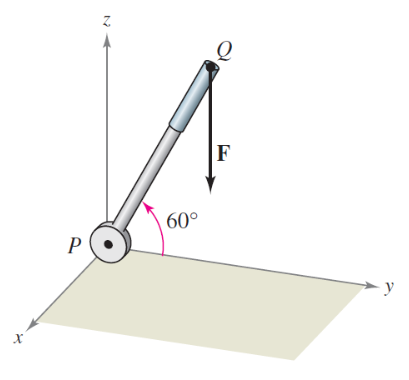
\includegraphics[width = .5\textwidth]{example4fig.png}&
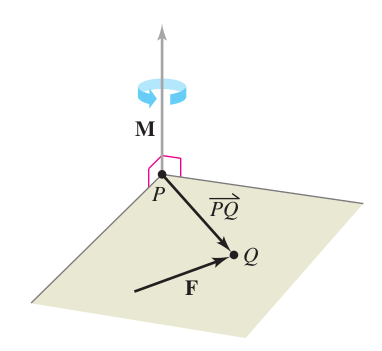
\includegraphics[width = .5\textwidth]{torque.png}
\end{tabular}\pause
\begin{tcolorbox}
$\mathbf M\text{ (or ${\tau}$)} = \overrightarrow{PQ}\times\mathbf F.$
\end{tcolorbox}
\pause
{\bf Remark: The torque is a vector, NOT a number.}
\end{frame}
\begin{frame}
\frametitle{Knowledge Check}
\begin{tcolorbox}
{\bf Determinants}:
\begin{itemize}
\item
$\begin{vmatrix}
u_1 &u_2\\
v_1&v_2
\end{vmatrix}=\pause u_1v_2 - u_2v_1.
$
\item
\begin{align*}
\begin{vmatrix}
u_1 &u_2&u_3\\
v_1&v_2&v_3\\
w_1&w_2&w_3
\end{vmatrix}
 &= \onslide<3->{ u_1\begin{vmatrix}
v_2&v_3\\
w_2&w_3
\end{vmatrix} - u_2\begin{vmatrix}
v_1&v_3\\
w_1&w_3
\end{vmatrix}  + u_3 \begin{vmatrix}
v_1&v_2\\
w_1&w_2
\end{vmatrix}\\
&=\onslide<4->{u_1(v_2w_3 - v_3w_2) - u_2(v_1w_3 - v_3w_1)\\
&\quad + u_3(v_1w_2 - v_2w_1).}}
\end{align*}
\end{itemize}
\end{tcolorbox}
\end{frame}

\begin{frame}
\frametitle{Knowledge Checks}

\only<1->{
Let $\mathbf u = u_1\mathbf i + u_2\mathbf j + u_3\mathbf k$ { and } $\mathbf v = v_1\mathbf i + v_2\mathbf j + v_3\mathbf k$ be vectors in space.
\begin{align*}
\mathbf u\times\mathbf v &:=
\begin{vmatrix}
\mathbf i&\mathbf j&\mathbf k\\
u_1&u_2&u_3\\
v_1&v_2&v_3
\end{vmatrix}=\begin{vmatrix}
u_2&u_3\\
v_2&v_3
\end{vmatrix}\mathbf i - \begin{vmatrix}
u_1&u_3\\
v_1&v_3
\end{vmatrix}\mathbf j+\begin{vmatrix}
u_1&u_2\\
v_1&v_2
\end{vmatrix}\mathbf k\\
&= (u_2v_3 - u_3v_2)\mathbf i - (u_1v_3 - u_3v_1)\mathbf j + (u_1v_2-u_2v_1)\mathbf k.
\end{align*}
}
\end{frame}

\begin{frame}
\frametitle{Triple scalar product}
\begin{figure}
\centering
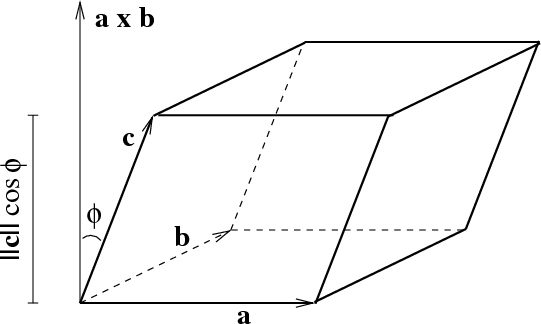
\includegraphics[width=.65\textwidth]{volume_parallelepiped.png}
\end{figure}
\begin{align*}
&\text{Volume(parallelepiped)}\onslide<2->{ = \abs{\norm{\mathbf a\times\mathbf b} \norm{\mathbf c}\cos\theta} } \onslide<3->{= \abs{\mathbf c\cdot \norm{\mathbf a\times\mathbf b}}}\\
\onslide<4->{
=&\ \abs{c_1(a_2b_3 - a_3b_2) - c_2(a_1b_3 - a_3b_1) + c_3(a_1b_2 - a_2b_1)}\\
=&\ \text{absolute value}\left(\begin{vmatrix}
c_1 &c_2&c_3\\
a_1&a_2&a_3\\
b_1&b_2&b_3
\end{vmatrix}\right)
}
\end{align*}
\end{frame}

\begin{frame}
\frametitle{The Right Hand Rule}
\begin{figure}
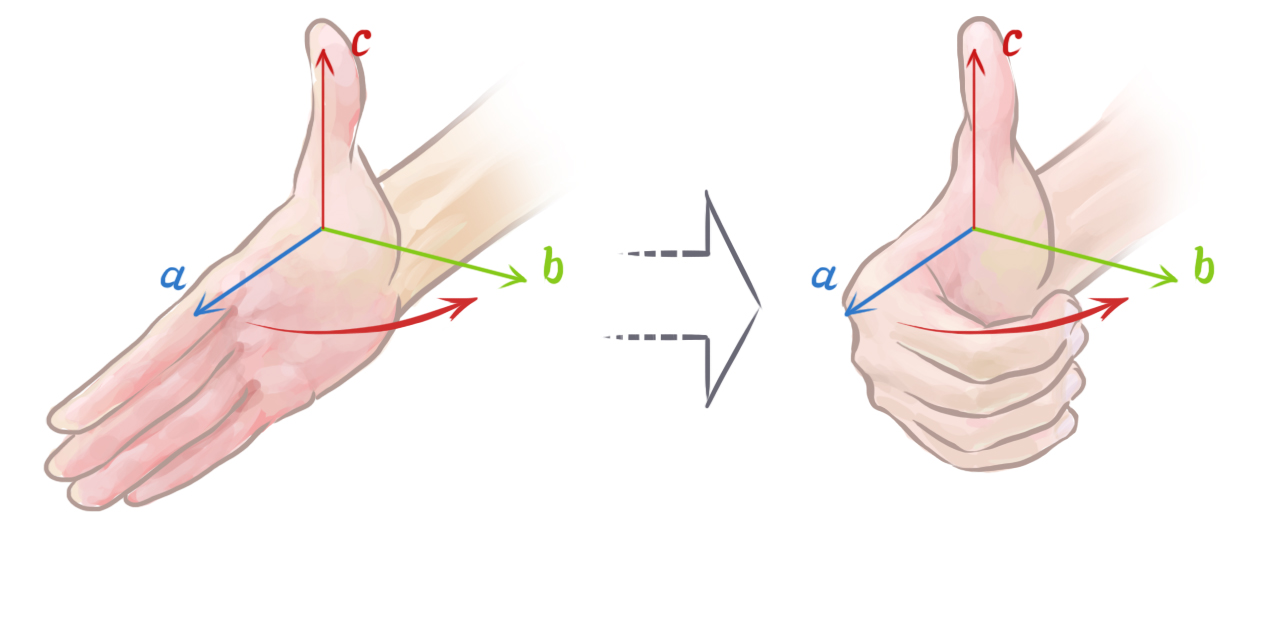
\includegraphics[width = .65\textwidth]{righthandrule1.png}
\end{figure}
\begin{tabular}{cc}
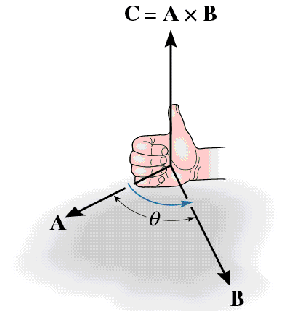
\includegraphics[width = .35\textwidth]{righthandrule2.png}&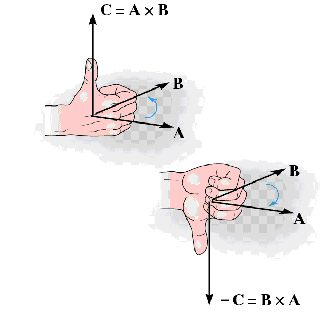
\includegraphics[width = .35\textwidth]{righthandrule3.png}
\end{tabular}
\end{frame}

\begin{frame}
\frametitle{The Cross Product of the Standard Unit Vectors}
{\bf Exercise.} According to the right hand rule and the magnitude formula, find 
\begin{itemize}[label = $\bullet$]
\item $\mathbf i\times\mathbf j$.
\item $\mathbf j\times\mathbf i$.
\item $\mathbf j\times\mathbf k$.
\item $\mathbf k\times\mathbf j$.
\item $\mathbf k\times\mathbf i$.
\item $\mathbf i\times\mathbf k$.
\end{itemize}
\end{frame}

\begin{frame}
\frametitle{The General Formula}
Suppose $\mathbf u = u_1\mathbf i + u_2\mathbf j + u_3\mathbf k$, $\mathbf v = v_1\mathbf i + v_2\mathbf j + v_3\mathbf k$. If distributivity is to be respected, we must have the following.\pause
\begin{align*}
\mathbf u \times \mathbf v =& \left(u_1\mathbf i + u_2\mathbf j + u_3\mathbf k\right)\times \left(  v_1\mathbf i + v_2\mathbf j + v_3\mathbf k\right)\\
=&\onslide<3->{\quad u_1v_1\mathbf i\times\mathbf i + u_1v_2\mathbf i\times\mathbf j + u_1v_3\mathbf i\times\mathbf k\\}
&\onslide<4->{+u_2v_1 \mathbf j\times\mathbf i  + u_2v_2 \mathbf j\times\mathbf j + u_2v_3 \mathbf j\times\mathbf k\\}
&\onslide<5->{+u_3v_1 \mathbf k\times\mathbf i + u_3v_2\mathbf k\times\mathbf j + u_3v_3\mathbf k\times\mathbf k\\}
\onslide<6->{=&\quad (u_2v_3 - u_3v_2)\mathbf i + (u_3v_1 - u_1v_3)\mathbf j + (u_1v_2 - u_2v_1)\mathbf k.}
\end{align*}
\end{frame}

\begin{frame}
\frametitle{Pin Support}
\begin{figure}[h]
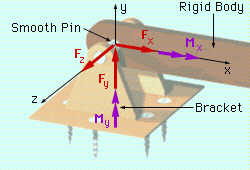
\includegraphics[width = 0.5\textwidth]{pinSupport.jpg}
\end{figure}
Suppose a force $\mathbf F = 2\mathbf i - 3\mathbf j + \mathbf k$ is acting on the lever at $(1,1,1)$. 
\begin{itemize}[label = $\bullet$]
\item
Find the torque of $\mathbf  F$ about the origin.
\item If the lever is stuck, find the force $\inpr{F_x, F_y, F_z}$ at the pin support.
\item If the lever can rotate freely about pin, find the couple moment $\inpr{M_x, M_y, M_z}$ at the pin support.
\end{itemize}
\end{frame}

\end{document}